\begin{frame}
\frametitle{Introduction}
\begin{columns}
    \column[t]{5cm}
	\begin{figure}[htbp!]
		\begin{center}
			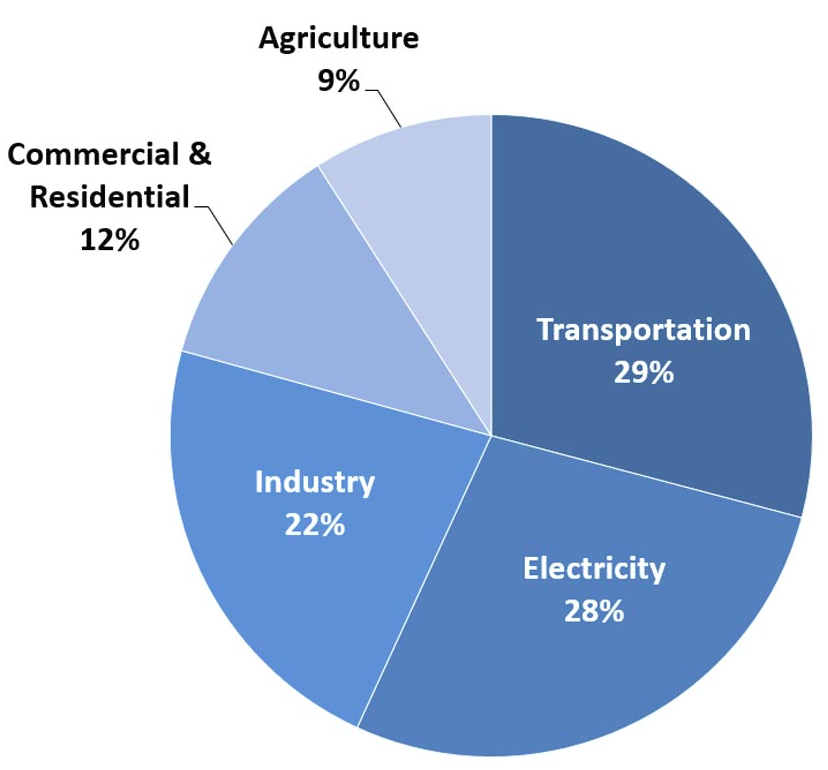
\includegraphics[height=6.2cm]{images/total-ghg-2017.png}
		\end{center}
		\caption{Total U.S. GHG Emissions by Economic Sector in 2017 \cite{us_epa_sources_2020}.}
	\end{figure}

	\column[t]{5cm}
	\begin{itemize}
		\item Illinois Climate Action Plan (iCAP).
		\item Attain carbon neutrality by 2050.
	\end{itemize}
\end{columns}
\end{frame}

% Notes:
% Transportation and Electricity are the economic sectors that produced ...

\begin{frame}
\frametitle{Transportation}
\begin{columns}
	\column[t]{5cm}
	\begin{itemize}
		\item Hydrogen economy
		\item california, japan, germany
	\end{itemize}

% Maybe a figure?
 %    \column[t]{5cm}
	% \begin{figure}[htbp!]
	% 	\begin{center}
	% 		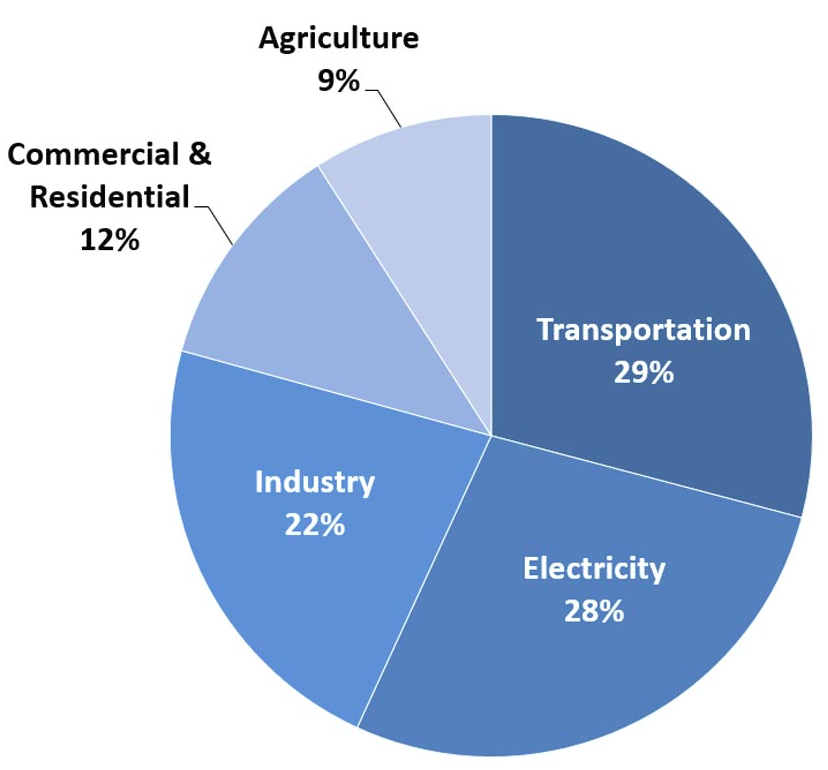
\includegraphics[height=6.2cm]{images/total-ghg-2017.png}
	% 	\end{center}
	% 	\caption{Total U.S. GHG Emissions by Economic Sector in 2017 \cite{us_epa_sources_2020}.}
	% \end{figure}
\end{columns}
\end{frame}

\begin{frame}
\frametitle{Electricity}
\begin{columns}
	\column[t]{5cm}
	\begin{itemize}
		\item More renewables
		\item Duck curve
	\end{itemize}

% Maybe a figure?
 %    \column[t]{5cm}
	% \begin{figure}[htbp!]
	% 	\begin{center}
	% 		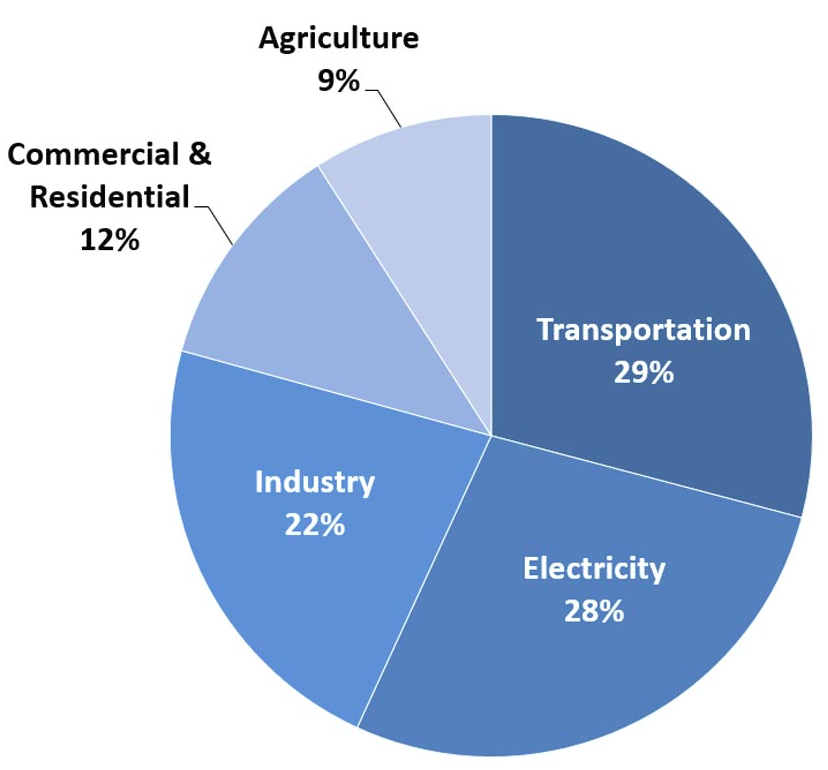
\includegraphics[height=6.2cm]{images/total-ghg-2017.png}
	% 	\end{center}
	% 	\caption{Total U.S. GHG Emissions by Economic Sector in 2017 \cite{us_epa_sources_2020}.}
	% \end{figure}
\end{columns}
\end{frame}

















% \begin{frame}
% \frametitle{"There must be something wrong at SL-1"}
% \begin{columns}
%     \column[t]{5cm}
% 	\begin{itemize}
% 		\item 9:01 pm alarm goes off at the main firehouse.
% 		\item Radiation readings too high, no signs of the crew.
% 		\item Ed Vallario went inside and saw Jack Byrnes.
% 		\item Retrieval of Byrnes and finding  of Legg.
% 		\item Byrnes was pronounced dead at 11:14 PM.
% 		\item Another group found the 3rd member pinned to the roof.
% 	\end{itemize}

%     \column[t]{5cm}
% 	\begin{itemize}
%         \item Retrieval of Legg's body.
%         \item Retrieval of McKinley's body.
%         \item Bodies taken to processing plant.
% 	\end{itemize}

%     "We got a reading on the detector, that by todays' standards, you'd have gotten the hell out of there." \textit{Lamprecht}.
%     \\
%     "I went to take a breath and it was like there was no more oxygen in the tank." \textit{Vallario}.

% \end{columns}
% \end{frame}

% \begin{frame}
% \frametitle{The accident}
% \begin{columns}
%     \column[t]{5cm}
% 	\begin{figure}[htbp!]
% 		\begin{center}
% 			\includegraphics[height=4.5cm]{./images/crew1a.png}
% 		\end{center}
% 		\caption{Reactor crew positions before the accident \cite{mckeown2003idaho}.}
% 	\end{figure}

%     \column[t]{5cm}
% 	\begin{itemize}
% 		\item Central rod is withdrawn 20".
% 		\item Reactor goes critical at 16.7".
% 		\item Fuel plates vaporize, water gets to 3740$^{\circ}$ F.
% 		\item Center fuel elements and central control blade ejected.
% 		\item Vessel rises out of its sheat and hits the ceiling.
% 		\item Vessel falls down.
% 	\end{itemize}
% \end{columns}
% \end{frame}


% \begin{frame}
% \frametitle{Theories}

% ”The direct cause of the incident clearly appears to have been the manual withdrawal by one or more of the maintenance crew of the central control rod blade from the SL-1 core considerably beyond the limit specified in the maintenance procedure. The reason or motive for the abnormal withdrawal is considered highly speculative, and it does not appear at all likely that there will ever be any reasons to change this judgment.”

% \end{frame}

% \begin{frame}
% \frametitle{Evaluation}
% 	\begin{block}{Author and Audience}
% 		\begin{itemize}
% 			\item Sources: Interviews and official documents.
% 			\item Wide audience.
% 		\end{itemize}
% 	\end{block}

% 	\begin{block}{Technical Evaluation}
% 		\begin{itemize}
% 			\item Technical explanation is not too extensive.
% 			\item A lot of details on the post-accident procedures.
% 			\item Description of the autopsies is extremely detailed.
% 		\end{itemize}
% 	\end{block}

% 	\begin{block}{Non-Technical Evaluation}
% 		\begin{itemize}
% 			\item Anecdotes, feelings, and opinions.
% 			\item Several theories on why Byrnes pulled from the rod.
% 			\item Verifiability is lost.
% 		\end{itemize}
% 	\end{block}
% \end{frame}